\documentclass[11pt]{article}
\usepackage[margin=1in]{geometry}
\usepackage{amsmath}
\usepackage{amssymb}
\usepackage{hyperref}
\usepackage{tikz}
\usetikzlibrary{arrows.meta,positioning,shapes,fit}

\title{Context-Aware FinCommerce Pipeline}
\author{}
\date{January 21, 2026}

\begin{document}
\maketitle

\section*{Overview}
This report summarizes the end-to-end Context-Aware FinCommerce Recommendation Pipeline, including schema setup, data generation, vector insertion, and semantic search with reranking.

\section*{Pipeline Diagram}
\begin{center}
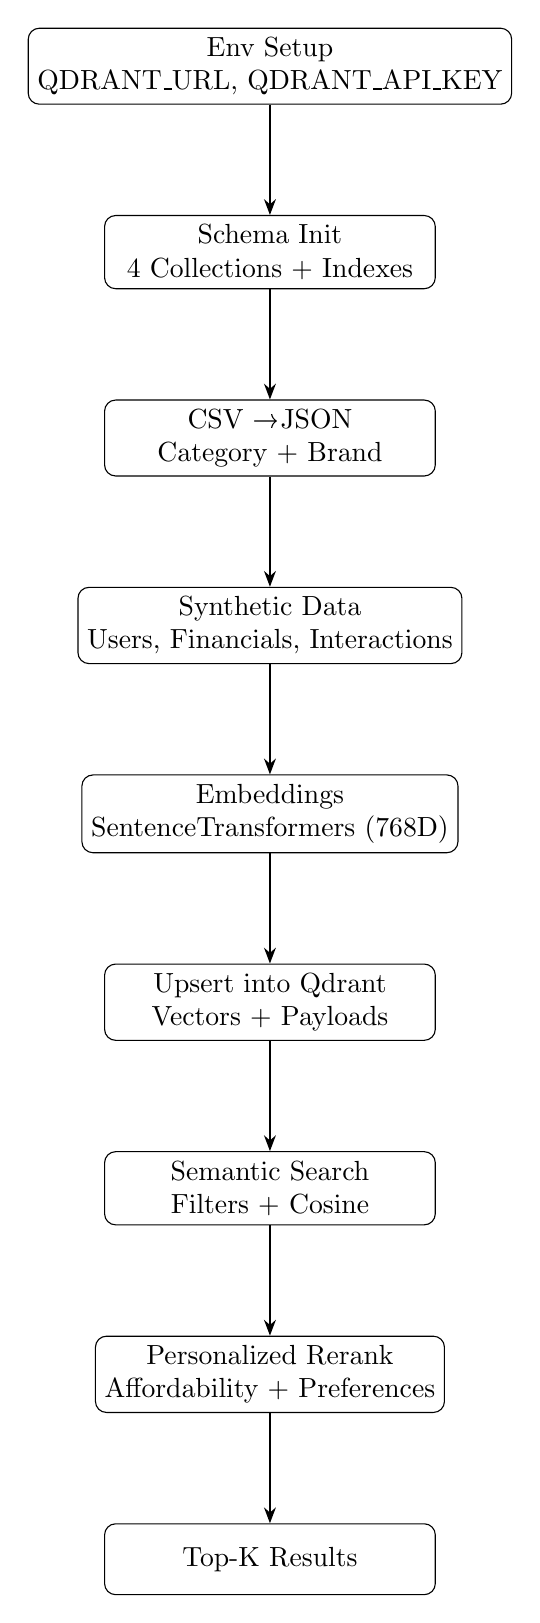
\begin{tikzpicture}[
  node distance=1.4cm,
  box/.style={rectangle, rounded corners, draw=black, align=center, minimum width=4.2cm, minimum height=0.9cm},
  arrow/.style={-{Stealth[length=2mm]}, thick}
]

\node[box] (env) {Env Setup\\QDRANT\_URL, QDRANT\_API\_KEY};
\node[box, below=of env] (schema) {Schema Init\\4 Collections + Indexes};
\node[box, below=of schema] (payload) {CSV \textrightarrow JSON\\Category + Brand};
\node[box, below=of payload] (gen) {Synthetic Data\\Users, Financials, Interactions};
\node[box, below=of gen] (embed) {Embeddings\\SentenceTransformers (768D)};
\node[box, below=of embed] (upsert) {Upsert into Qdrant\\Vectors + Payloads};
\node[box, below=of upsert] (search) {Semantic Search\\Filters + Cosine};
\node[box, below=of search] (rerank) {Personalized Rerank\\Affordability + Preferences};
\node[box, below=of rerank] (output) {Top-K Results};

\draw[arrow] (env) -- (schema);
\draw[arrow] (schema) -- (payload);
\draw[arrow] (payload) -- (gen);
\draw[arrow] (gen) -- (embed);
\draw[arrow] (embed) -- (upsert);
\draw[arrow] (upsert) -- (search);
\draw[arrow] (search) -- (rerank);
\draw[arrow] (rerank) -- (output);

\end{tikzpicture}
\end{center}

\section*{Score Contribution Visualization}
\begin{center}
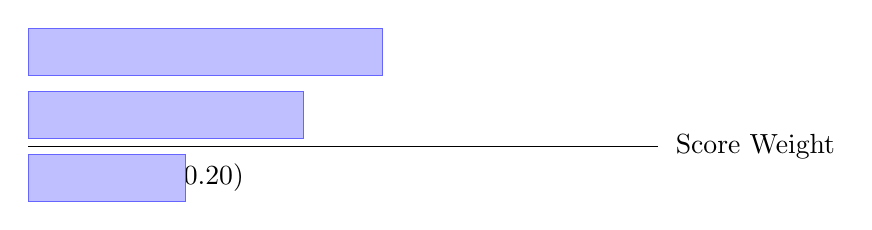
\begin{tikzpicture}[
  bar/.style={fill=blue!25, draw=blue!60, minimum height=0.6cm},
  label/.style={anchor=west},
  axis/.style={draw=black}
]

% Axis
\draw[axis] (0,0) -- (8,0);
\node[anchor=west] at (8.1,0) {Score Weight};

% Bars (scaled by weight * 10)
\node[label] at (0,1.2) {Semantic (0.45)};
\node[bar] at (2.25,1.2) [minimum width=4.5cm] {};

\node[label] at (0,0.4) {Affordability (0.35)};
\node[bar] at (1.75,0.4) [minimum width=3.5cm] {};

\node[label] at (0,-0.4) {Preference (0.20)};
\node[bar] at (1.0,-0.4) [minimum width=2.0cm] {};

\end{tikzpicture}
\end{center}

\section*{Core Scoring Formula}
\[
\text{final\_score} = 0.45\, s_{\text{semantic}} + 0.35\, s_{\text{afford}} + 0.20\, s_{\text{pref}}
\]

\[
 s_{\text{afford}} = \begin{cases}
0, & \text{if } \text{available\_balance} \le 0 \\
\max\left(0, 1 - \frac{\text{price}}{\text{available\_balance}}\right), & \text{otherwise}
\end{cases}
\]

\[
 s_{\text{pref}} = \max\left(\mathbb{1}[\text{category} \in \text{preferred\_categories}],\ \mathbb{1}[\text{brand} \in \text{preferred\_brands}]\right)
\]

\section*{Key Collections}
\begin{itemize}
  \item \textbf{products\_multimodal} (768D): price, category, brand, in\_stock, region
  \item \textbf{user\_profiles} (768D): location, risk\_tolerance
  \item \textbf{financial\_contexts} (256D): available\_balance, credit\_limit, eligible\_installments
  \item \textbf{interaction\_memory} (768D): user\_id, purchased
\end{itemize}

\section*{Execution Summary}
\begin{enumerate}
  \item Setup Qdrant collections and payload indexes.
  \item Transform transactional CSV into product JSON payloads.
  \item Generate synthetic user, financial, and interaction data.
  \item Generate 768D embeddings using SentenceTransformers for text fields.
  \item Upsert all points into Qdrant.
  \item Query using semantic similarity with price and stock filters.
  \item Rerank by affordability and preferences.
  \item Return top-$k$ ranked products.
\end{enumerate}

\end{document}
